\subsection{Ancient Egypt: Where Math Was Actually Useful}

In ancient Egypt, mathematics was a government job. You can thank the Nile River for that. Every year, the river flooded, wiping out property lines like a chaotic, unregulated HOA.  

This led to the invention of surveyors, also known as the \textit{harpedonaptae} (literally “rope stretchers”), who used ratios to put the land back together.  

The harpedonaptae didn’t have laser levels or GPS satellites. What they had were ropes, stakes, and math; and somehow, they made it work. Their ropes were knotted at regular intervals, which allowed them to create proportional lengths and consistent angles. It was like ancient trigonometry, but without the sines, cosines, or existential dread of taking a calc final.

\begin{figure}[H]
\centering
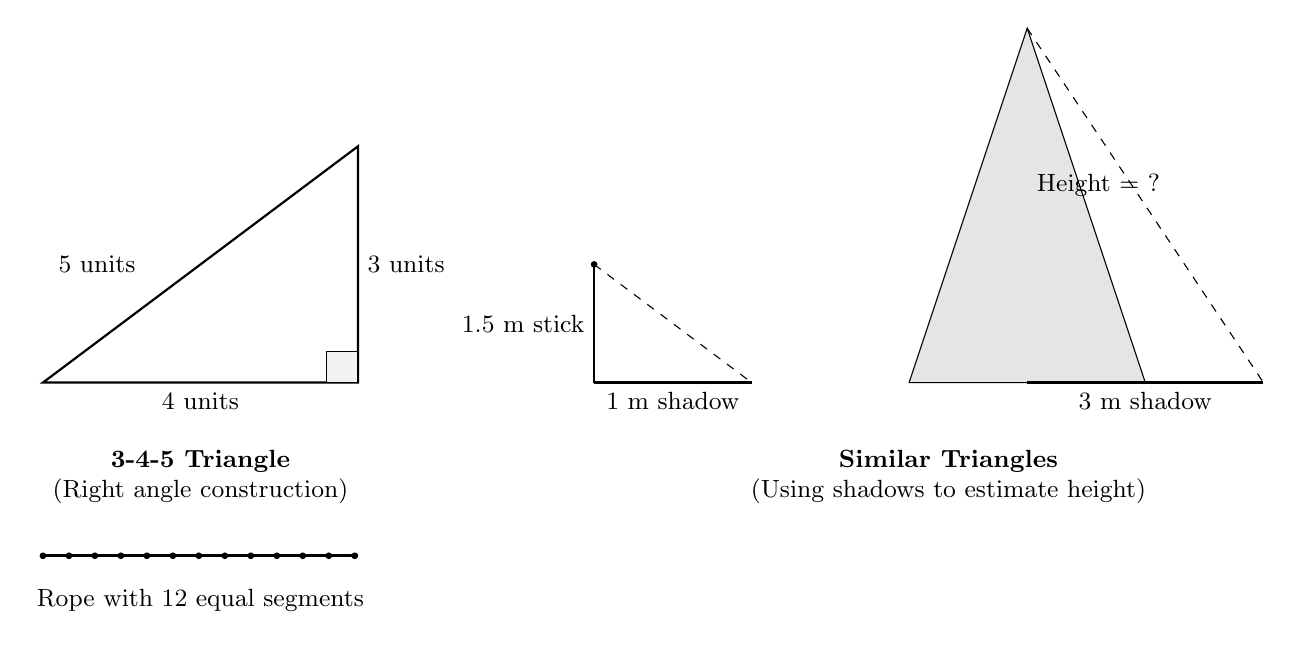
\begin{tikzpicture}[scale=1, every node/.style={font=\small}]

% --- 3-4-5 Triangle (Left) ---
\draw[thick] (0,0) -- (4,0) -- (4,3) -- cycle;
\draw[fill=gray!10] (4,0) rectangle (3.6,0.4);

\node[below] at (2,0) {4 units};
\node[right] at (4,1.5) {3 units};
\node[left] at (1.3,1.5) {5 units};
\node[align=center] at (2,-1.2) {\textbf{3-4-5 Triangle} \\ (Right angle construction)};

% Rope depiction
\foreach \i in {0,...,12} {
  \filldraw[black] ({\i*0.33}, -2.2) circle (1pt);
}
\draw[very thick, black] (0,-2.2) -- (4,-2.2);
\node[below] at (2,-2.5) {Rope with 12 equal segments};

% --- Similar Triangles (Right) ---
% Small stick and shadow
\draw[thick] (7,0) -- (7,1.5); % stick
\draw[thick] (7,0) -- (9,0); % shadow
\draw[dashed] (7,1.5) -- (9,0); % hypotenuse
\filldraw[black] (7,1.5) circle (1pt);
\node[left] at (7,0.75) {1.5 m stick};
\node[below] at (8,0) {1 m shadow};

% Pyramid and its shadow
\draw[fill=gray!20] (11,0) -- (12.5,4.5) -- (14,0) -- cycle; % pyramid
\draw[thick] (12.5,0) -- (15.5,0); % shadow
\draw[dashed] (12.5,4.5) -- (15.5,0); % hypotenuse
\node[below] at (14,0) {3 m shadow};
\node[right] at (12.5,2.5) {Height = ?};

% Labels
\node[align=center] at (11.5,-1.2) {\textbf{Similar Triangles} \\ (Using shadows to estimate height)};

\end{tikzpicture}
\caption{Left: The \textbf{3-4-5 triangle} used by the \textit{harpedonaptae} to construct right angles. \\
Right: \textbf{Shadow ratio trick}—if a 1.5-meter stick casts a 1-meter shadow, and a pyramid casts a 3-meter shadow, then by similar triangles, the pyramid is 4.5 meters tall.}
\end{figure}


They used the principle of similar triangles to measure inaccessible lengths. Want to figure out the width of the Nile without swimming across and possibly being eaten by a crocodile? Simple: plant a stick in the ground, measure its shadow, then compare it to the shadow of something else (like a pyramid, a tree, or your boss). The ratio of shadow to height stays the same --- assuming the sun isn’t gaslighting you that day.

Need to mark out a right angle? Tie a rope into 12 equal segments, form a triangle with sides 3, 4, and 5, and bam --- congrats, you’ve just built a right triangle. You might not get a medal, but you can now draw a rectangular field without anyone accusing you of witchcraft. 

In essence, these rope-stretching wizards turned geometry into a practical survival skill. Where modern surveyors use high-tech tools and CAD software, the harpedonaptae used proportional reasoning to tame the chaos of nature --- and occasionally, the Nile.



At this point, math was still firmly rooted in the real world. And it could have stayed that way.  

But then the Greeks got involved.  

\begin{figure}[H]
\centering
\begin{tikzpicture}[every node/.style={font=\footnotesize}]

% Panel 1 — Egyptian surveyor doing land ratios
\comicpanel{0}{4}
  {Surveyor}
  {Farmer}
  {Your new field is 2 units long and 1 unit wide. Congrats, you now own a rectangle.}
  {(0,-0.5)}

% Panel 2 — Engineer using ratios
\comicpanel{6.5}{4}
  {Engineer}
  {Foreman}
  {If the base is twice the height, the ramp won’t collapse. Probably.}
  {(0,-0.5)}

% Panel 3 — Egyptian priest estimating golden ratio
\comicpanel{0}{0}
  {Priest}
  {Apprentice}
  {If we keep this ratio, the pyramid looks divine. Or at least intimidating.}
  {(0,0.8)}

% Panel 4 — Greek philosopher enters
\comicpanel{6.5}{0}
  {Greek}
  {Everyone}
  {What if numbers aren’t just useful, but… beautiful?}
  {(0,0.8)}

\end{tikzpicture}
\caption{Egyptians used ratios to measure fields. Greeks used them to measure the soul.}
\end{figure}